\label{sec:Versuch2.2.1}
Dieser Versuchsteil befasst sich mit der grafischen Darstellung der Momentanleistung mithilfe eines Oszilloskopes. Der Verlauf von Strom und Spannung, deren Phasenverschiebung zueinander und der Zusammenhang zum Verlauf der Momentanleistung werden betrachtet.


\subsubsection{Versuchsaufbau}
\label{sec:Aufbau2.2.1}

Abbildung \ref{fig:Plan2-1} zeigt den in diesem Versuchsteil verwendeten Schaltplan. Die Impedanzen $Z_1$ und $Z_2$ sind einstellbar, $Z_1 = 0uF, 1uF, \cdots, 10uF$, $Z_2 =  0\Omega, 10\Omega, \cdots, 100\Omega$ Folgende Werte werden verwendet:
\begin{itemize}
\item $Z_1 = \frac{1}{j\omega C} \mbox{ mit } C=4\mu F$
\item $Z_2 = 60\Omega$
\item $Z_3 = R_{sp} + j\omega L$ mit $R_{sp} = 5,5\Omega; L=15,84mH$
\item $u_{ges}$ wird durch Veränderung von $R_I$ auf 6V eingestellt.
\end{itemize}

\begin{figure}[h]
\centering
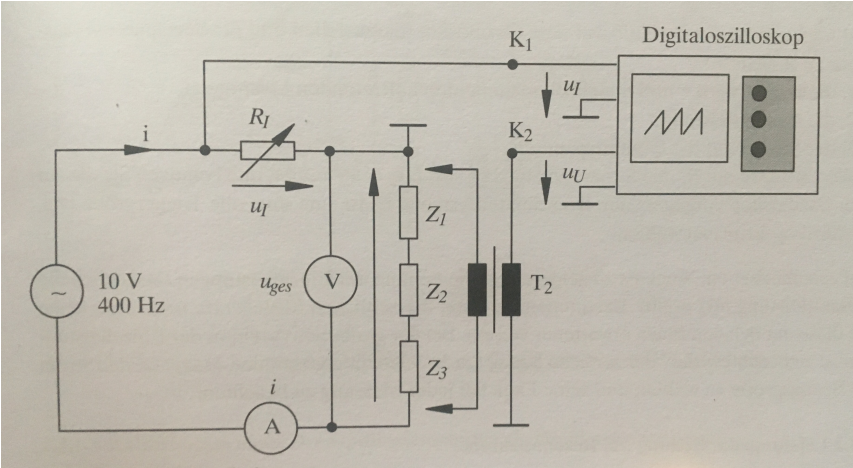
\includegraphics[width=0.7\linewidth]{Images/Aufbau2-1.png}
\caption{Schaltplan Versuch 2.1, \cite[47]{GEMLBuch}}
\label{fig:Plan2-1}
\end{figure}

Im Folgenden wird das Oszilloskop zur Anzeige der Momentanleistung verwendet. Hierfür wird die Spannung über einen beliebigen Verbraucher mithilfe des potentialtrennenden Transformators $T_2$ am Oszilloskopeingang gemessen. Der Transformator ist notwendig, um den Referenzpunkt der zu messenden Spannung frei wählen zu können. Da seine Übersetzung 1:1 entspricht beeinflusst er die Spannung nicht weiter. Der Strom $i$ wird anhand der am Widerstand $R_I$ abfallenden Spannung gemessen. Zusätzlich lässt sich der Effektivwert des Stromes am Ampermeter ablesen.

Das Oszilloskop nun wird so eingestellt, dass das Produkt aus $u_I$ und $u_U$ angezeigt wird. Da $u_I$ proportional zu $i$ ist wird so eine zur Momentanleistung proportionale Kurve angezeigt.

\subsubsection{Auswertung der Momentanleistungskurven}

Die im Folgenden dargestellten Kurven werden vom Oszilloskop abgespeichert. \textit{Ch~1} (blaue Kurve) stellt hierbei die zum Strom proportionale Kurve dar, \textit{Ch~2} (rote Kurve) die am Verbraucher gemessene Spannung. Die Momentanleistung $p(t)$ wird durch die grüne Kurve dargestellt.
\\
Folgende Kurven werden gemessen:

\paragraph{Momentanleistung am Kondensator}
Sie ist in Abbildung \ref{fig:MomLKurveZ1} dargestellt. Deutlich zu sehen ist die Phasenverschiebung von Strom und Spannung, welche bei ca. $\frac{\pi}{2}$ liegt. Die Kurve der Momentanleistung schwingt mit doppelter Frequenz um 0, besitzt also keinen Gleichanteil. Dies entspricht genau der Vorhersage von Gleichung \eqref{eq:MomLeistungSplit} bzw. \eqref{eq:LeistungGleichanteil}, welche für eine Phasenverschiebung von $\varphi_u - \varphi_i = -\frac{\pi}{2}$, wie sie beim Kondensator vorliegt, eine rein sinusförmige Schwingung und keine Wirkleistung vorhersagen. Der Kondensator nimmt somit entsprechend Gleichung \eqref{eq:KomplexS} eine Leistung von $\underline{S} = UIe^{-i\frac{\pi}{2}}$ auf.\par

\begin{figure}[H]
\centering
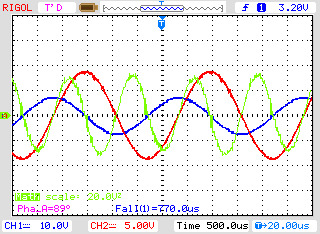
\includegraphics[width=0.7\linewidth]{Oszi-Bitmaps/NewFile0.jpg}
\caption{Momentanleistung am Kondensator. $u_I(t)$ (Blau), $u_{Z1}(t)$ (Rot), $p_{Z_1}(t)$ (Grün)}
\label{fig:MomLKurveZ1}
\end{figure}

\paragraph{Momentanleistung am Ohm'schen Widerstand}
Die Kurve der an einem Ohm'schen Widerstand gemessenen Momentanleistung ist in Abbildung \ref{fig:MomLKurveZ2} zu sehen. Da es sich um einen Verbraucher mit rein realer Impedanz handelt, gibt es keine Phasenverschiebung zwischen $u(t)$ und $i(t)$. Dies ist deutlich in der Grafik zu erkennen. Entsprechend Gleichung \eqref{eq:MomLeistungSplit} sollte die Kurve der Momentanleistung für $\varphi_u = \varphi_i$ rein positiv sein und einen deutlichen Gleichanteil von $UI$ besitzen. Auch dies ist in der Grafik klar erkennbar. Der Widerstand nimmt also konstant Leistung auf, es wird keine Leistung abgegeben. Entsprechend Gleichungen \eqref{eq:LeistungGleichanteil} und \eqref{eq:LeistungBlindanteil} ist die Wirkleistung maximal, die Blindleistung minimal.


\begin{figure}[H]
\centering
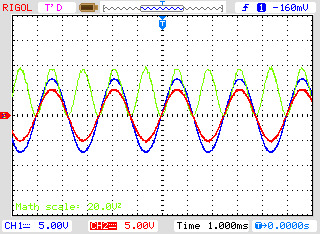
\includegraphics[width=0.7\linewidth]{Oszi-Bitmaps/NewFile1.jpg}
\caption{Momentanleistung am Ohm'schen Widerstand. $u_I(t)$ (Blau), $u_{Z2}(t)$ (Rot), $p_{Z_2}(t)$ (Grün)}
\label{fig:MomLKurveZ2}
\end{figure}

\paragraph{Momentanleistung an einer Spule}
Die Kurve der an einer Spule mit nicht-vernachlässigbarem Innenwiderstand ($R_{sp} = 5.5\Omega)$ gemessenen Momentanleistung ist in Abbildung \ref{fig:MomLKurveZ3} zu sehen. Ähnlich wie beim Kondensator (Abbildung \ref{fig:MomLKurveZ1}) ist eine Phasenverschiebung zwischen Strom und Spannung zu sehen. Diese ist jedoch etwas kleiner als die für eine reine Induktivität erwarteten $\frac{\pi}{2}$, welches sich durch den Innenwiderstand erklären lässt. Durch eine Komplexe Impedanz von $\underline{Z} = R_{sp} + j\omega L = 5.5\Omega + j39.81\Omega$ lässt sich eine Phasenverschiebung von $arc(\underline{Z}) = 82.134^\circ$ erwarten. Dies stimmt in etwa mit der Messung des Oszilloskopes überein. Entsprechend Gleichung \eqref{eq:MomLeistungSplit} sollte die Kurve der Momentanleistung einen kleinen Gleichanteil von etwa $P = \cos(\varphi)\cdot S=0.136\cdot S$ besitzen. Auch dies lässt sich in der Abbildung erkennen. Dennoch überwiegt entsprechend Gleichung \eqref{eq:LeistungBlindanteil} die Blindleistung der Spule mit $Q=\sin(\varphi)\cdot S=0.99\cdot S$.

\begin{figure}[H]
\centering
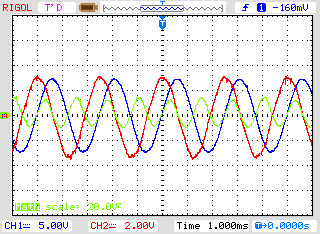
\includegraphics[width=0.7\linewidth]{Oszi-Bitmaps/NewFile2.jpg}
\caption{Momentanleistung an einer Spule mit Innenwiderstand. $u_I(t)$ (Blau), $u_{Z3}(t)$ (Rot), $p_{Z_3}(t)$ (Grün)}
\label{fig:MomLKurveZ3}
\end{figure}

\paragraph{Momentanleistung der gesamten Schaltung}
Die Kurve der in der gesamten Schaltung verbrauchten Momentanleistung ist in Abbildung \ref{fig:MomLKurveGesamt} zu erkennen. Da es sich hier um eine beliebig zusammengesetzte komplexe Impedanz handelt, lässt sich direkt keine Vorhersage über den Verlauf der Momentanleistung formulieren. Der hohe Gleichanteil legt jedoch nahe, dass die am Widerstand abfallende Leistung überwiegt. Die Phasenverschiebung lässt sich aus der Grafik als $\varphi = -\frac{\pi}{4}$ ablesen und stimmt der obigen Vermutung zu.
Durch Summierung der Impedanzen der Komponenten lässt sich die Gesamtimpedanz berechnen:
\begin{eqnarray}
\underline{Z}_{ges} =& \sum_{\mu=1}^3\underline{Z}_\mu = 65.5\Omega - j59.66\Omega\\
\mbox{Arg}(\underline{Z}) =& -42.33^\circ
\end{eqnarray}
Die berechnete Phasenverschiebung entspricht hier also fast genau der anhand der Abbildung geschätzten Verschiebung.

Entsprechend Gleichungen \eqref{eq:LeistungGleichanteil} und \eqref{eq:LeistungBlindanteil} ist es also tatsächlich so, dass Blind- und Scheinleistung hier etwa den gleichen Betrag von $\sin(45^\circ)\cdot S=\cos(45^\circ)\cdot S = \frac{1}{\sqrt{2}} \cdot S$ besitzen.

\begin{figure}[H]
\centering
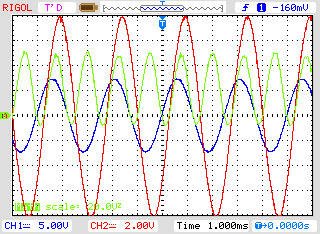
\includegraphics[width=0.7\linewidth]{Oszi-Bitmaps/NewFile3.jpg}
\caption{Momentanleistung der gesamten Schaltung. $u_I(t)$ (Blau), $u_{ges}(t)$ (Rot), $p_{ges}(t)$ (Grün)}
\label{fig:MomLKurveGesamt}
\end{figure}

\subsubsection{Grafische Addition der Leistung}
Es wird zusätzlich überprüft, ob sich die Momentanleistung der einzelnen Impedanzen addieren lassen, um die Momentanleistung des gesamten Systemes zu erhalten. Hierfür werden für einige beliebig gewählte Phasenwinkel die Werte der Momentanleistung aus den Oszilloskop-Messungen abgelesen und miteinander verglichen. Die Ergebnisse hierfür sind in Tabelle \ref{tab:Momentanleistungswerte} zu sehen.

Abgesehen von einer leichten Diskrepanz bei $\varphi = 90^\circ$ welche durch die Ungeauigkeit beim Ablesen erklärt werden kann, gleicht sich die Summe der einzelnen Momentanleistungen mit der im gesamten System verbrauchten Leistung. Dies ist auch mathematisch zu erwarten, da gilt:
\begin{eqnarray*}
& \underline{S}_{ges} =& \underline{U}_{ges}\cdot\underline{I}^* \\
\Leftrightarrow &\underline{S}_{ges} =& \underline{Z}_{ges}\cdot\underline{I}\cdot\underline{I}^* = \underline{Z}_{ges}\cdot |\underline{I}|^2 \\
\Leftrightarrow & \underline{S}_{ges} =& \underbrace{(\underline{Z}_1 + \underline{Z}_2 + \underline{Z}_3)}_{Z_{ges}} \cdot |\underline{I}|^2 \\
\Leftrightarrow & \underline{S}_{ges} =& \sum_{\mu=1}^3 \underbrace{\left(\underline{Z}_\mu \cdot |\underline{I}|^2\right)}_{S_\mu}\\
\end{eqnarray*}